\documentclass{article}
\usepackage[utf8]{inputenc}
\usepackage{amsmath,amsthm,amssymb}
\usepackage{listings}
\usepackage{pgfplots}
\usepackage{graphicx}
\usepackage{listings}
\usepackage{float}
%\usepackage{ctex}
\newtheorem*{claim}{Claim}
\newtheorem{theorem}{Theorem}
\title{Performance Programming}
%\author{Wenqi Tu}
\date{}
\lstset{frame=tb,
	language=C,
	aboveskip=3mm,
	belowskip=3mm,
	showstringspaces=false,
	columns=flexible,
	basicstyle={\small\ttfamily},
	numbers=none,
	numberstyle=\tiny\color{gray},
	keywordstyle=\color{blue},
	%commentstyle=\color{dkgreen},
	%stringstyle=\color{mauve},
	breaklines=true,
	breakatwhitespace=true,
	tabsize=3
}
\begin{document}


\section{problem description}

The main step of the MD model is the $evolve$ function.The $evolve$
function is a loop with the follow steps as bellow:
\begin{enumerate}
\item set the viscosity term in the force calculation for each dimension:
\begin{equation}\label{viscosity}
	f[i]=-vis[i]\times velo[i],i=0,1,\cdots,N-1
\end{equation}
\item add the wind term in the force calculation for each dimension:
\begin{equation}\label{wind}
f[i]=f[i]-vis[i]\times b,i=0,1,\cdots,N-1
\end{equation}
\item calculate distance from central mass:
\begin{equation}\label{distance}
	r[i]=\sqrt{pos[0][i]^{2}+pos[1][i]^{2}+pos[2][i]^{2}}
\end{equation}
\item calculate central force for each dimension:
\begin{equation}\label{centralforce}
	f[i]=f[i]-\frac{G\times mass[i]\times M\_central\times pos[i]}{r[i]^{3}}
\end{equation}
\item calculate pairwise separation of the particles for each dimension:$delta\_pos$
\item calculate norm of separation vector: %
$$delta\_r[k]=\sqrt{delta\_pos[0][k]^{2}+delta\_pos[1][k]^{2}+delta\_pos[2][k]^{2}}$$
\item add pairwise forces
\item update positions $pos[j][i]=pos[j][i]+dt*velo[j][i]$
\item update velocities:$velo[j][i]=velo[j][i]+dt*(f[j][i]/mass[i])$
\end{enumerate}

\section{performance profile}

Before do the optimization, we need to profile the $MD$ application.We
use Intel advisor to profile the performance.The roofline of the application
is given as bellow:
\begin{figure}[H]
	\centering
	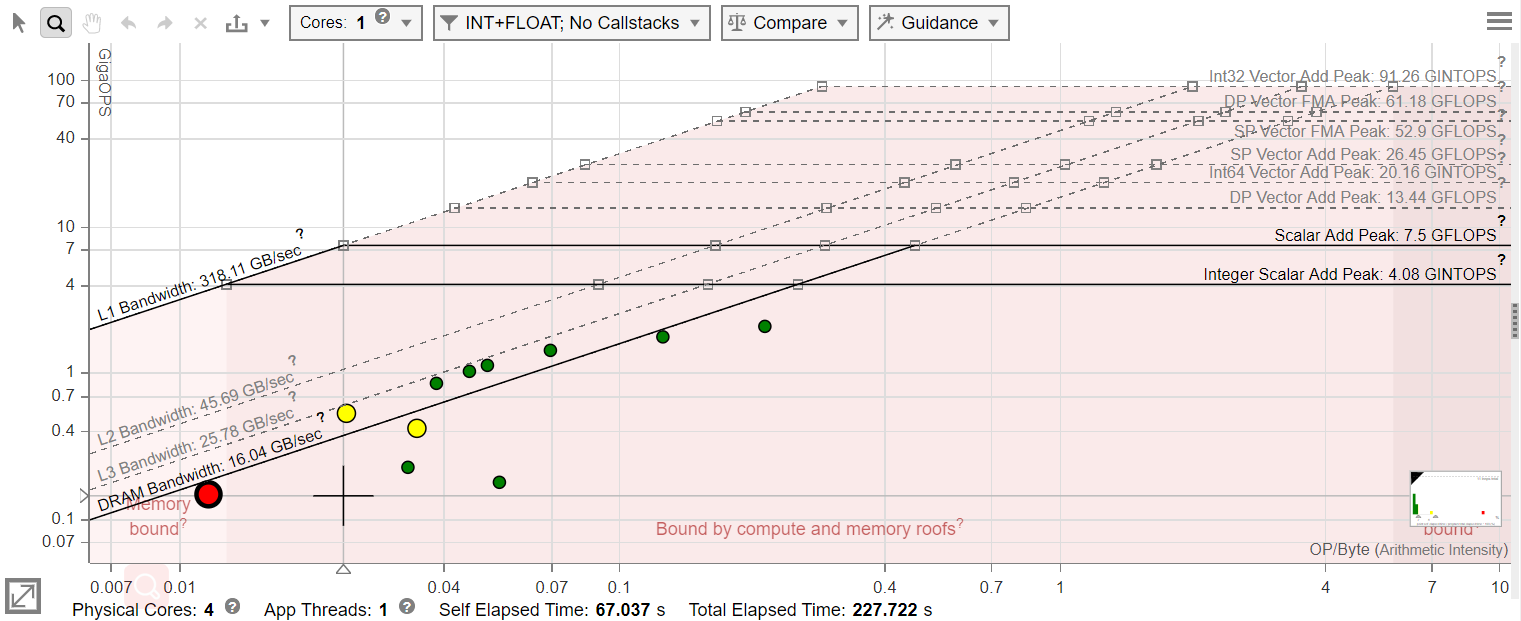
\includegraphics[width=0.7\linewidth]{roofline}
	\caption{roofline of the MD application}
	\label{fig:roofline}
\end{figure}



\noindent from the roofline figure, we can get that the bottle-neck
of the application is bounded by memory. we have get that the main
process of the application is the $evolve$ function. The elapsed
time of the code in $evolve$ function is given as bellow (descending
order):
\begin{figure}[H]
	\centering
	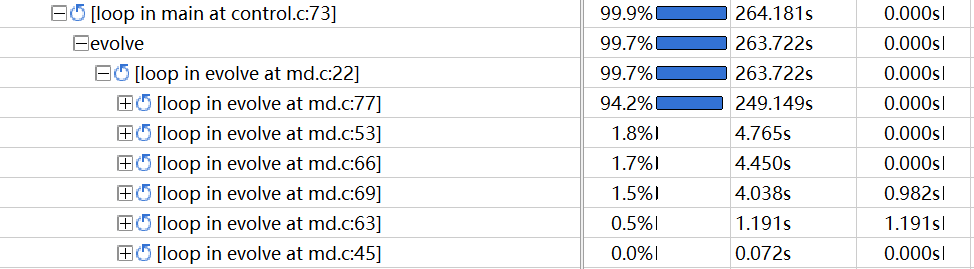
\includegraphics[width=0.7\linewidth]{time.jpg}
	\caption{$evolve$ function elapsed time diftribution (descending order)}
	\label{fig:time}
\end{figure}


\noindent From Fig.\ref{fig:time} we can get that the bottle-neck of the application is the code in $md.c$ line 77, Then in order to get more details, we get the figure from $intel\quad advisor$ and given as bellow:
\begin{figure}[H]
	\centering
	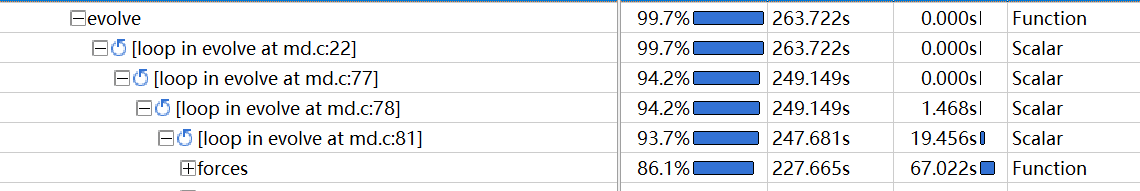
\includegraphics[width=0.7\linewidth]{force.jpg}
	\caption{the bottle-neck of the code is the function $force$}
	\label{fig:force}
\end{figure}
\section{optimization}
From the performace profile part, we can get that the application is bounded by memory, and the $force$ function is the bottle-neck of the application. So our optimization will include the tips bellow:
\begin{enumerate}
	\item focus on bottle-neck then do other optimization
	\item merge some operations into one loop to reduce memory read and write
	\item change the order of the loop to increase memory cache hit
	\item optimize the force function.
	\item reduce logical branches jump time.
	\item reduce repeat operation
\end{enumerate}
\subsection{bottle-neck optimization}
\noindent First the  $force$ function is 
\begin{lstlisting}[caption={force function}]{H}
	double forces(double Wv, double deltav, double rv){
		return Wv*deltav/(pow(rv,3.0));
	}
\end{lstlisting}
We can get that the operation $pow(rv,3.0)$ is much slower than  the operation $rv*rv*rv$, so the new $force$ function is 
\begin{lstlisting}[caption={modified force function}]{H}
	double forces(double Wv, double deltav, double rv){
		return Wv*deltav/(rv*rv*rv);
	}
\end{lstlisting}
\subsubsection{reduce logical branches and reduce Redundant operation}
From Fig.\ref{fig:time} we can get that the bottle-neck of the application is the code in $md.c$ line 77, the code is given as bellow:
\begin{lstlisting}{H}
for(i=0;i<Nbody;i++)
{
	for(j=i+1;j<Nbody;j++)
	{
		size = radius[i] + radius[j];
		have_collided=0;
		for(l=0;l<Ndim;l++)
		{
			/*  flip force if close in */
			if( delta_r[k] >= size )
			{
				f[l][i] = f[l][i] -
				forces(G*mass[i]*mass[j],delta_pos[l][k],delta_r[k]);
				f[l][j] = f[l][j] + 
				forces(G*mass[i]*mass[j],delta_pos[l][k],delta_r[k]);
			}
			else
			{
				f[l][i] = f[l][i] + 
				forces(G*mass[i]*mass[j],delta_pos[l][k],delta_r[k]);
				f[l][j] = f[l][j] - 
				forces(G*mass[i]*mass[j],delta_pos[l][k],delta_r[k]);
				have_collided=1;
			}
		}
		if( have_collided == 1 )
		collisions++;
		k = k + 1;
	}
}
\end{lstlisting}
From the code we can get that the logical branch for $if(delta\_r[k]>=size)$ can put outside the third loop. And as for the $collisions++$ operation, we can remove the $if( have_collided == 1 )$ branch, and add it into the $else$ branch of the code. Then as to the $force$ operation in the branch, its all the same operation, so we can just do it only once.  

Then as to $forces(G*mass[i]*mass[j],delta_pos[l][k],delta_r[k])$, we can get that each inner loop only change is $delta_pos[l][k]$, so we can spilt the operation into two steps
\begin{lstlisting}[caption={split force into two steps}]{H}
	double G_mass_r3 = G * mass[i] * mass[j] / (delta_r[k] * delta_r[k] * delta_r[k]);
	gravitation = G_mass_r3*delta_pos[l][k];
\end{lstlisting}
So we can get that for the bottle-neck of this part after optimization is :
\begin{lstlisting}[caption={split force into two steps}]{H}
double gravitation;
for(i=0;i<Nbody;i++)
{
	for(j=i+1;j<Nbody;j++)
	{
		size = radius[i] + radius[j];
		double G_mass_r3 = G * mass[i] * mass[j] / (delta_r[k] * delta_r[k] * delta_r[k]);
		if (delta_r[k] >= size)
		{
			for (l = 0; l < Ndim; l++)
			{
				gravitation = delta_pos[l][k] * G_mass_r3;
				f[l][i] -= gravitation;
				f[l][j] += gravitation;
			}
		}
		else
		{
			for (l = 0; l < Ndim; l++)
			{
				gravitation = delta_pos[l][k] * G_mass_r3;
				f[l][i] += gravitation;
				f[l][j] -= gravitation;
			}
		collisions++;}
		k = k + 1;}}
\end{lstlisting}
\subsection{merge operation and unroll loop}
From the equation eq.\eqref{viscosity}  eq.\eqref{wind} eq.\eqref{distance} eq.\eqref{centralforce}, we can get that the 4 steps will visit the array $f$ many times, but if we use unroll and merge the 4 equations into one, will just need to visit $f$ only once. and for the distance variable $r$, we nolonger need to visit the $r$ array, we just use a temp variable replace. So the 4 equations code after optimization is given as bellow:
\begin{lstlisting}[caption={loop unroll and merge the 4 equations}]{H}
for (i = 0; i < Nbody; i++)
{
	double tmp = sqrt(pos[0][i] * pos[0][i] + pos[1][i] * pos[1][i] + pos[2][i] * pos[2][i]);
	tmp = G * mass[i] * M_central / (tmp*tmp*tmp);
	f[0][i] = -vis[i] * (velo[0][i] + wind[0]) - tmp* pos[0][i];
	f[1][i] = -vis[i] * (velo[1][i] + wind[1]) - tmp* pos[1][i];
	f[2][i] = -vis[i] * (velo[2][i] + wind[2]) - tmp* pos[2][i];
}
\end{lstlisting}
the steps 5,6,7 in section 1 is compute $delta\_pos$ and $delta_r$, then use $delta\_pos$ and $delta_r$ to compute pairwise forces. so we can also merge the three steps into one. So we can merge the steps 5,6 and the code in $Listing\quad 4$ into one loop. the optimized code is given as bellow:
\begin{lstlisting}[caption={merge steps 5,6,7 into one step}]{H}
k = 0;
double delta_r_k;
double gravitation;
double tmp_pos[Ndim];
double tmp_fli[Ndim];
for(i=0;i<Nbody;i++)
{

	for (l = 0; l < Ndim; l++)
	{
		tmp_pos[l] = pos[l][i];
		tmp_fli[l] = f[l][i];
	}
	for(j=i+1;j<Nbody;j++)
	{
		delta_pos[0][k] = tmp_pos[0] - pos[0][j];
		delta_pos[1][k] = tmp_pos[1] - pos[1][j];
		delta_pos[2][k] = tmp_pos[2] - pos[2][j];
		
		delta_r_k = sqrt(delta_pos[0][k] * delta_pos[0][k] +
		delta_pos[1][k] * delta_pos[1][k] +
		delta_pos[2][k] * delta_pos[2][k]);
		size = radius[i] + radius[j];
		double G_mass_r3 = G * mass[i] * mass[j] / (delta_r_k * delta_r_k * delta_r_k);
		if (delta_r_k >= size)
		{
			for (l = 0; l < Ndim; l++)
			{
				gravitation = delta_pos[l][k] * G_mass_r3;
				tmp_fli[l] -= gravitation;
				f[l][j] += gravitation;
			}
		}
		else
		{
			for (l = 0; l < Ndim; l++)
			{
				gravitation = delta_pos[l][k] * G_mass_r3;
				tmp_fli[l] += gravitation;
				f[l][j] -= gravitation;
			}
			collisions++;
		}
		k = k + 1;
	}
	for (l = 0; l < Ndim; l++)
	f[l][i] = tmp_fli[l];
}
\end{lstlisting}
From the code, we can get that in-order to reduce the visit time of $pos[l][i]$ and $f[l][i]$, we store them in two tmp array $tmp\_pos$
and $tmp\_fli$
\subsection{merge update positions and velocities into one loop}
for the positions and velocities can be compute in one loop (steps 8,9), then we merge them into one loop and in order to reduce cache hit, we use unroll. the optimized code is given as bellow:
\begin{lstlisting}[caption={merge steps 8,9 into one step}]{H}
	for(i=0;i<Nbody;i++)
	{
		pos[0][i] =  pos [0][i] + dt * velo[0][i];
		velo[0][i] = velo[0][i] + dt * (f[0][i] / mass[i]);
		
		pos[1][i] = pos[1][i] + dt * velo[1][i];
		velo[1][i] = velo[1][i] + dt * (f[1][i] / mass[i]);
		
		pos[2][i] = pos[2][i] + dt * velo[2][i];
		velo[2][i] = velo[2][i] + dt * (f[2][i] / mass[i]);
	}
\end{lstlisting}
\section{correctness check and result}
\subsection{correctness check}
for the original application is so slow, when we do the correctness check, we set $Nsteps =50,Nsave=5$ to do the correctness check. We use $diff-output$ to compare the output data. We can find that the original application result and the optimized application result is all the same.
\subsection{summary}
We can get that the original application includes 9 steps from section 1. But after the optimization, the application only includes 3 steps
\begin{enumerate}
	\item calculate the central force for each dimension
	\item add pairwise forces
	\item update positions and velocities
\end{enumerate}
To optimize the code, the skill we use is unroll loop, merge operations, reduce logical branches, reduce memory access, change the order of loop, use multiply to replace $pow$ operation.
\subsection{compare the performance}
\begin{enumerate}
\item 250 timesteps took 21.814722 seconds for \textbf{optimized code}
\item 250 timesteps took 995.058564 secondss for \textbf{original code}

\end{enumerate}
So we can get that the optimized code is 50 faster than the original code.
\subsection{test platform}
\begin{enumerate}
\item compile tool : gcc
\item cpu : i7-8550U CPU @ 1.80GHz
\item system: ubuntu 
\item profile tool: intel advisor
\end{enumerate}
\end{document}
